\subsection{Teorija odločanja}

\begin{naloga}{?}{Vaje OR 30.3.2016}
\begin{vprasanje}
Na ulici nas ustavi neznanec in nam predlaga met kovanca.
Če pade grb, nam izplača $250000 €$,
če pade glava, pa mi njemu $100000 €$.
Ali naj sprejmemo ponudbo?

\end{vprasanje}
\begin{odgovor}
\end{odgovor}
\end{naloga}


\begin{naloga}{Batagelj, Kaufman}{\cite[Naloga~4.2]{bk}}
\begin{vprasanje}
Trgovina pri pekarni kupuje žemlje po $0.2 €$
in jih prodaja po $0.4 €$.
Skozi leta poslovanja so izračunali naslednjo porazdelitev za prodajo žemljic.
\begin{center}
\begin{tabular}{c|cccccc}
Prodaja & $50$ & $60$ & $70$ & $80$ & $90$ & $100$ \\
\hline
Verjetnost & $0.1$ & $0.15$ & $0.3$ & $0.2$ & $0.15$ & $0.1$
\end{tabular}
\end{center}
Če žemelj zmanjka, naročijo pri pekarni razliko,
pri čemer jih žemlja tedaj stane $0.3 €$.
Ob koncu dneva jim pekarna odkupi presežek po $0.15 €$ na žemljo.
Koliko žemelj se trgovini splača kupiti?

\end{vprasanje}
\begin{odgovor}
\end{odgovor}
\end{naloga}


\begin{naloga}{?}{Izpit OR 5.6.2014}
\begin{vprasanje}
Pacient ima na voljo operacijo.
Brez operacije bo živel natanko $3$ mesece.
Z uspešno opravljeno operacijo bo živel natanko $12$ mesecev.
Operacija je neuspešna z verjetnostjo $0.3$
(v tem primeru pacient dočaka $0$ mesecev).
Cilj pacienta je maksimiranje pričakovane življenjske dobe.
\begin{enumerate}[(a)]
\item Ali naj pacient sprejme operacijo?
\item Pacient lahko opravi predhodni test,
ki z zanesljivostjo $0.9$ napove uspeš\-nost operacije,
vendar z verjetnostjo $0.005$ pacient zaradi komplikacij med testom umre.
Ali naj pacient opravi test?
\end{enumerate}
Nariši odločitveno drevo
in odločitve sprejmi na podlagi izračunanih ve\-rjet\-no\-sti!
\end{vprasanje}
\begin{odgovor}
\end{odgovor}
\end{naloga}


\begin{naloga}{?}{Vaje OR 30.3.2016}
\begin{vprasanje}
Podjetje je razvilo produkt,
za katerega je konkurenca pripravljena plačati $15 \ME$.
Če se odločijo samostojno prodajati produkt,
jih vzpostavitev proizvodnje stane $6 \ME$,
za vsak uspešno prodan produkt pa dobijo $600 €$.
Računajo, da bi z verjetnostjo $0.5$ investicija uspela
in bi prodali $100000$ produktov,
z verjetnostjo $0.5$ pa bi projekt propadel
in bi prodali zgolj $10000$ produktov.
Podjetje se lahko odloči tudi za neodvisno raziskavo trga.
Ta stane $1 \ME$,
z verjetnostjo $2/3$ pa bo pravilno napovedala uspeh projekta
(ne glede na to, ali bi ta uspel ali ne).
Kako naj se podjetje odloči?

\end{vprasanje}
\begin{odgovor}
\end{odgovor}
\end{naloga}


\begin{naloga}{?}{Izpit OR 24.6.2015}
\begin{vprasanje}
Veliki koncert skupine FiM
se bo odvijal v dvorani s $100$ neoznačenimi sedeži.
Prireditelj se lahko odloči, da proda $100$, $101$, $102$ ali $103$ karte
(povpraševanja je dovolj).
Znane so verjetnosti $p_0 = 0.2$, $p_1 = 0.3$, $p_2 = 0.4$ in $p_3 = 0.1$,
kjer je $p_i$ verjetnost, da $i$ kupcev kart ne pride na koncert
(ne glede na število prodanih kart).
Vsaka prodana karta prinese $10 €$ dobička,
vsak obiskovalec, ki ne bo mogel v dvorano, pa pomeni $30 €$ stroškov
(ker je že plačal $10 €$ za karto, ima torej organizator $20 €$ izgube).
Koliko kart naj prireditelj proda, da bo pričakovani dobiček čim večji?

\end{vprasanje}
\begin{odgovor}
\end{odgovor}
\end{naloga}


\begin{naloga}{?}{Kolokvij OR 31.5.2012}
\begin{vprasanje}
Rexhep Bajrami bi se rad naslednja štiri leta
ukvarjal s prodajo sadja in zelenjave
(po štirih letih mu poteče delovna viza).
Rad bi najel parcelo za stojnico, ki bo stala $6000 €$.
Če je lokacija dobra, bo imel $12000 €$ dobička,
če pa je lokacija slaba, bo imel le $3000 €$ dobička.
Ocenjuje, da je z verjetnostjo $2/3$ lokacija dobra,
z verjetnostjo $1/3$ pa slaba.
\begin{enumerate}[(a)]
\item Z odločitvenim drevesom opiši njegove možnosti in ugotovi,
kako naj se odloči ter kakšen dobiček naj pričakuje.
\item Za nasvet lahko vpraša znanca Seada, ki ``ima nos'' za tovrstne posle.
Sead mu lahko da nasvet, a zanj zahteva $1200 €$.
Dobro je znano, da ima Sead naslednje pogojne verjetnosti
$P(\text{Seadovo mnenje} \; | \; \text{kakovost parcele})$:
\begin{center}
\begin{tabular}{c|cc}
& dobra & slaba \\
\hline
priporoča & $2/3$ & $1/2$ \\
odsvetuje & $1/3$ & $1/2$
\end{tabular}
\end{center}
Ali naj vpraša Seada za nasvet?
Kakšen je pričakovani dobiček?
\end{enumerate}
\end{vprasanje}
\begin{odgovor}
\end{odgovor}
\end{naloga}


\begin{naloga}{Sergio Cabello}{Izpit OR 15.3.2017}
\begin{vprasanje}[nal:dectree]
Imaš odločitveno drevo s slike~\ref{fig:dectree},
a nisi prepričan glede vrednosti $p \in [0, 1/3]$.
Poišči optimalne odločitve glede na vrednost $p$.

\begin{figure}[t]
	\centering
	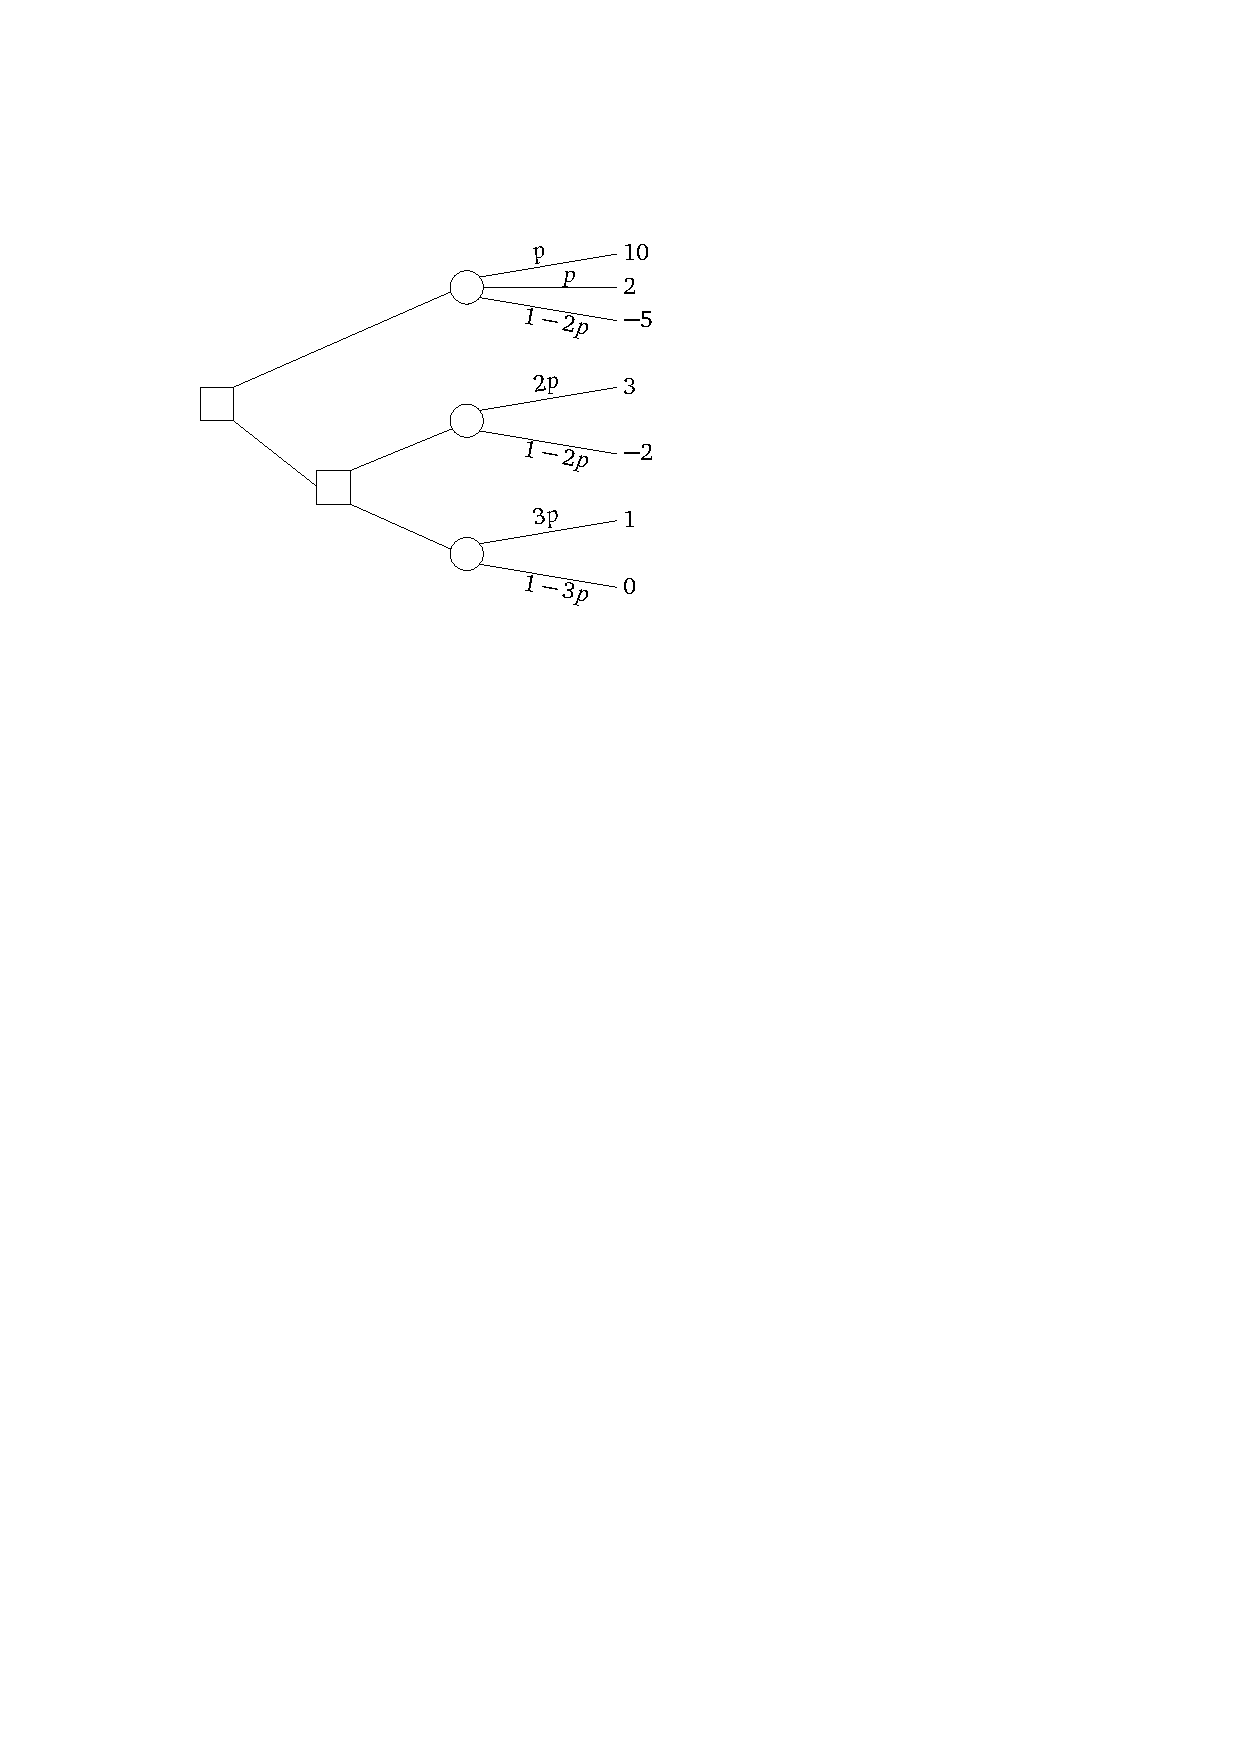
\includegraphics{slike/decision-tree.pdf}
    \caption{Odločitveno drevo za nalogo~\ref{nal:dectree}.}
    \label{fig:dectree}
\end{figure}

\end{vprasanje}
\begin{odgovor}
\end{odgovor}
\end{naloga}


\begin{naloga}{Janoš Vidali}{Izpit OR 15.12.2016}
\begin{vprasanje}[nal:avtobus]
Mudi se ti na izpit, a ravno v trenutku,
ko prideš na postajo Konzorcij, odpelje avtobus številka 1.
Na prikazovalniku se izpiše,
da bo naslednji avtobus številka 1 prispel čez $10$ minut,
naslednji avtobus številka 6 čez $6$ minut,
naslednji avtobus številka 14 pa čez $2$ minuti.

Avtobusa 1 in 6 ob ugodnih semaforjih potrebujeta $6$ minut do postaje pri FE,
pri čemer se lahko čas vož\-nje zaradi rdeče luči na semaforju pri FF
podaljša za $1$ minuto.
Verjetnosti, da bo rdečo luč imel avtobus 1, da bo rdečo luč imel avtobus 6,
ter da bosta oba avtobusa imela zeleno luč, so enake $1/3$
(zaradi majhnega razmaka se ne more zgoditi,
da bi oba avtobusa naletela na rdečo luč).
Avtobus številka 1 nadaljuje pot do postaje pri FMF,
za kar potrebuje še $2$ minuti.

Avtobus številka 14 potrebuje $5$ minut do postaje pri študentskih domovih,
od tam pa greš peš do postaje pri FE, za kar potrebuješ še $4$ minute.
Pri tem prečkaš že\-lez\-ni\-co -- če mimo pripelje vlak
(kar se zgodi z verjetnostjo $0.05$),
se čas hoje podaljša za $3$ minute.
Ko prideš na postajo pri FE
(ne glede na to, ali si prišel z avtobusom 6 ali 14),
te čakajo še $4$ minute hoje do FMF,
vendar moraš najprej prečkati Tržaško cesto.
Če je na semaforju rdeča luč
(kar se zgodi z verjetnostjo 0.9, neodvisno od drugih dogodkov),
se lahko odločiš, da $2$ minuti počakaš na zeleno luč in potem nadaljuješ peš,
ali pa da greš nazaj do postaje in počakaš na avtobus številka $1$
(ki bo, tako kot prej, vozil še $2$ minuti do FMF).

Kakšne bodo tvoje odločitve,
da bo pričakovano trajanje poti do FMF čim krajše?
Nariši od\-lo\-čit\-ve\-no drevo
in odločitve sprejmi na podlagi izračunanih verjetnosti!
Glej sliko~\ref{fig:avtobus} za shemo možnih poti.

\begin{figure}[t]
\centering
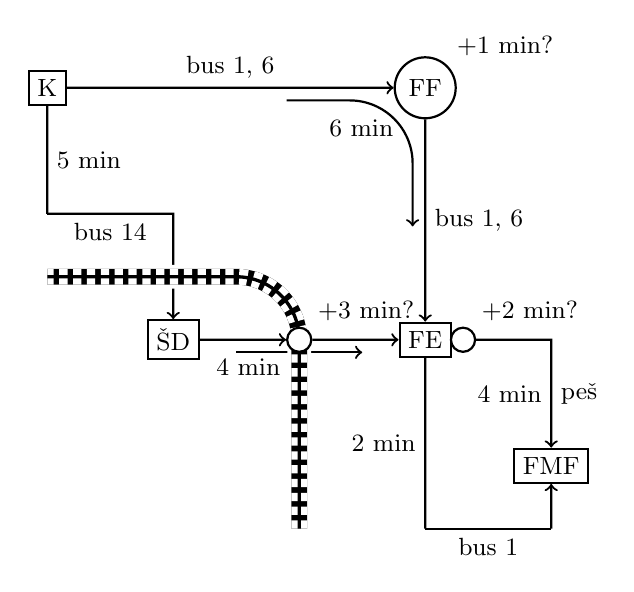
\begin{tikzpicture}[style=thick,scale=0.8]
\tikzstyle{vertex}=[draw, fill=white]
\small
\node[vertex,rectangle] (K)   at (-4, 3) {K};
\node[vertex,circle]    (FF)  at ( 2, 3) [label=45:$+1$ min?, label=225:$6$ min] {FF};
\node[vertex,rectangle] (SD)  at (-2,-1) {ŠD};
\node[vertex,rectangle] (FE)  at ( 2,-1) {FE};
\node[vertex,circle]    (FEs) at (2.6,-1) [label=45:$+2$ min?] {};
\node[vertex,rectangle] (FMF) at ( 4,-3) {FMF};

\draw[->] (K) -- (FF)
    node [midway, above] {bus 1, 6};
\draw (K) -- (-4, 1)
    node [midway, right] {$5$ min};
\draw (-4, 1) -- (-2, 1)
    node [midway, below] {bus 14};
\draw[->] (-4, 1) -- (-2, 1) -- (SD);
\draw[->] (FF) -- (FE)
    node [midway, right] {bus 1, 6};
\draw[->] (FEs) -- (4,-1) -- (FMF)
    node [midway, left] {$4$ min}
    node [midway, right] {peš};
\draw (FE) -- (2,-4)
    node [midway, left] {$2$ min};
\draw (2,-4) -- (4,-4)
    node [midway, below] {bus 1};
\draw[->] (4,-4) -- (FMF);

\draw[->] (-0.2,2.8) -- (0.8,2.8) arc (90:0:1) -- (1.8,0.8);
\draw[->] (-1,-1.2) -- (1,-1.2);

\draw[line width=3mm, white] (0,-4) -- (0,-1) arc (0:90:1) -- (-4, 0);
\draw[line width=2mm] (0,-4) -- (0,-1) arc (0:90:1) -- (-4, 0);
\draw[line width=2mm, white, densely dashed] (0,-4) -- (0,-1) arc (0:90:1) -- (-4, 0);
\draw[very thick] (0,-4) -- (0,-1) arc (0:90:1) -- (-4, 0);

\node[vertex,circle] (Z)   at ( 0,-1) [label=45:$+3$ min?, label=225:$4$ min] {};
\draw[->] (SD) -- (Z);
\draw[->] (Z) -- (FE);
\end{tikzpicture}
\caption{Shema možnih poti za nalogo~\ref{nal:avtobus}.}
\label{fig:avtobus}
\end{figure}
\end{vprasanje}
\begin{odgovor}
\end{odgovor}
\end{naloga}
